

    Object modeling methodologies such as Unified Modeling Language (UML) are becoming increasingly popular in both database and software design. These methodologies go beyond database design to specify detailed design of software modules and their interactions using various types of diagrams. Class diagrams are similar in many ways to the ER diagrams. In class diagrams, operations on objects are specified, in addition to specifying the database schema structure. Operations can be used to specify the functional requirements during database design.

\section{Using High-Level Conceptual Data Models for Database Design}
    
    \begin{figure}
        \centering
        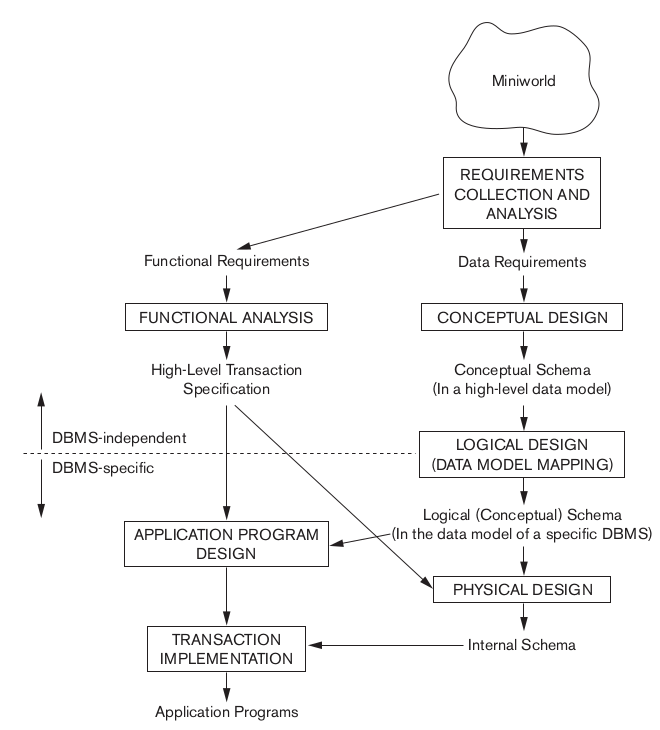
\includegraphics[scale=0.4]{chap3-1}
        \caption{A simplified diagram to illustrate the main phases of database design.}
        \label{fig:chap3-1}
    \end{figure}
    
    \textbf{Conceptual schema}: concise description of the data requirements of the users and includes detailed descriptions of the entity types, relationships, and constraints; these are expressed using the concepts provided by the high-level data model.
    
    \textbf{Logical design} or \textbf{data model mapping}: actual implementation of the database using
    a commercial DBMS, using an implementation data model - such as the relational (SQL) model - so the conceptual schema is transformed from the high-level data model into the implementation data model.
    
    \textbf{Physical design} phase: specify the internal storage structures, file organizations, indexes, access paths, and physical design parameters for the database files

\section{Entity Types, Entity Sets, Attributes,and Keys}
    \subsection{Entities and Attributes}
    \begin{itemize}
        \item \textbf{Entity}: thing or object in the real world with an independent existence
    May be an object with a physical existence (a particular person, car, house, or employee) or an object with a conceptual existence (a company, a job, or a university course). 
        \item \textbf{Attributes}: particular properties that describe an entity. 
    \end{itemize}
    
    \subsubsection{Attribute types}
    \begin{itemize}
        \item \textbf{Composite} attributes can be divided into smaller subparts (which can also be composite attributes (ex:street\_address $\rightarrow$ number, street)), which represent more basic attributes with independent meanings (ex: an address $\rightarrow$ street\_address, zip, city)
        \item \textbf{Simple} or \textbf{atomic} attributes cannot be divided.
        \item \textbf{Single-valued} attributes have a single value for a particular entity
        \item \textbf{Multivalued} attributes that can have a \textbf{set of values} or \textbf{domain} for the same entity (ex: colors of a car) (not represented on ER diagrams)
        \item \textbf{Derived} attributes can be determined by using one or more \textbf{stored} attributes or related entities (ex: \# of employees)
        \item \textbf{NULL values}: a particular entity may not have an applicable value (not applicable) or we don't know the value of that attribute (missing)
        \item \textbf{Complex} attributes are grouped composite attributes whose components are displayed using parentheses (), separated by commas and displaying multivalued attributes between braces \{\}
    \end{itemize}


\section{Entity Types, Entity Sets, Keys, and Value Sets}
\begin{itemize}
    \item \textbf{Entity type}: defines a collection (or set) of entities that have the same attributes (ex: Employee). Each entity type in the database is described by its name and attributes.
    
    \item \textbf{Entity set} or \textbf{entity collection}: collection of all entities of a particular entity type in the database, also called the extension of the entity type. (the entity set is usually referred to using the same name as the entity type, even though they are two separate concepts)
    
    \item An entity type describes the \textbf{schema} or \textbf{intension} for a set of entities that share the same structure. 
    
    \item \textbf{Uniqueness constraint} on attributes (or \textbf{key}). These attributes can be used to identify each entity uniquely. 
    \item \textbf{Composite key}: Several attributes together can form a key: the combination of the attribute values must then be distinct for each entity. To represent this in the ER model, define a composite attribute and designate it as a key attribute of the entity type. Composite keys must be \textbf{minimal}; that is, all component attributes must be included in the composite attribute to have the uniqueness property

    \begin{figure}
        \centering
        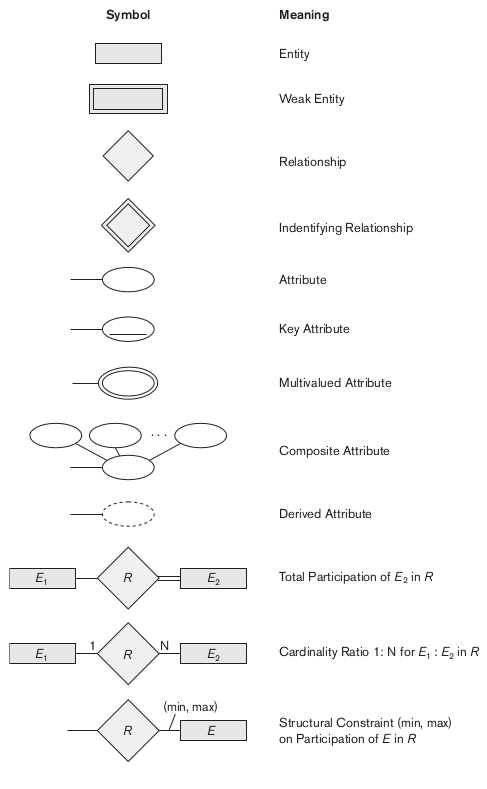
\includegraphics[scale=0.4]{chap3-14}
        \caption{Summary of the notation for ER diagrams.}
        \label{fig:chap3-14}
    \end{figure}
    
    \item \textbf{Weak entity type}: Entity type that has no key.


\section{Relationship Types, Relationship Sets, Roles, and Structural Constraints}
    \subsection{Relationship Types, Sets, and Instances}
    \paragraph{Book}
    A \textbf{relationship type} $R$ among $n$ entity types $E_1, E_2, ...E_n$ defines a set of associations—or a \textbf{relationship set}—among entities from these entity types. Both are referred by the same name $R$.
    
    Mathematically, the \textbf{relationship set} R is a set of \textbf{relationship instances} $r_i$, where each $r_i$ associates $n$ individual entities $(e_1,..,e_n)$ and each entity $e_j$ in $r_i$ is a member of the entity set $E_j$ ($1\leq j\leq n)$

    \paragraph{Slides}
    A \textbf{relation} represents the extension of some $n$-adic predicate P by having a body consisting of every $n$-tuple that satisfies P

    The corresponding mathematical intension could be: $$\{ < s, c > | \text{Student s is enrolled on course c} \}$$
    
    \begin{itemize}
        \item \textbf{Predicate}: The meaning of a certain kind of sentence, but often used (conveniently) to refer to the sentence itself.
        \item \textbf{Intension} of a predicate: its meaning (loosely speaking)
        \item \textbf{Extension} of a predicate: all the instantiations that are (believed to be) true.
        \item \textbf{Substitution}: replace a parameter by a designator
        \item \textbf{Instantiation}: substitution of all the parameters, yielding a proposition.
    \end{itemize}

    \paragraph{DEE and DUM}
    Relations corresponding to :
    \begin{itemize}
        \item $\{< > | 2 < 1\}$ : DUM (false)
        \item $\{< > | 2 > 1\}$ : DEE (true)
    \end{itemize}
    
    \begin{itemize}
        \item DUM is the relation that has no attributes and no tuples. It plays the role of False.
        \item DEE is the relation that has no attributes and a single tuple. It plays the role of True.
    \end{itemize}



    \subsection{Relationship Degree, Role Names, and Recursive Relationships}

    \begin{itemize}
        \item \textbf{Degree} of a relationship type: number of participating entity types (ex: binary, ternary, ...)
         \item \textbf{Recursive relationships} or \textbf{self-referencing relationships}: relationship in which the same entity type participates more than once but in different roles. (ex: employee and supervisor, which are both of type EMPLOYEE)
    \end{itemize}

    \subsection{Constraints on Binary Relationship Types}
    
    \begin{itemize}
        \item \textbf{Cardinality ratio}: specifies the \emph{maximum} number of relationship instances that an entity can participate in (ex: 1:1, 1:N, N:1, M:N)
        \item \textbf{Participation constraint} or \textbf{minimum cardinality constraint}: specifies the \emph{minimum} number of relationship instances that each entity can participate in. 2 kinds : total (or existence dependency) (\emph{double line}) and partial(\emph{single line}).
    \end{itemize}
    
    \subsection{Attributes of Relationship Types}
    Relationship types can also have attributes, similar to those of entity types. For example, to record the number of hours per week that a particular employee works on a particular project.
    
    \begin{itemize}
        \item Attributes of a 1:1 relationship type can be migrated to one of the participating entities
        \item Attributes of a 1:N relationship type can be migrated only to the entity type on the N-side
        \item Attributes of a M:N relationship type cannot be migrated and must have a dedicated relationship
    \end{itemize}
    
    Other (more precise) notation exists with (min, max)
    
    
\section{Weak entity types}

Entities belonging to a \textbf{weak} entity type are identified by being related(\textbf{identifying relationship}) to specific entities from another entity type(called \textbf{identifying} or \textbf{owner}) in combination with one of their attribute values.

A weak entity type always has a \emph{total participation constraint} with respect to its identifying relationship because a weak entity cannot be identified without an owner entity.

\begin{itemize}
    \item \textbf{Partial key}: attribute (may be composite, or all the weak entity's attributes) that can uniquely identify weak entities that are related to the same owner entity
\end{itemize}

\end{itemize}


